% Asset ID: A21FunctionsAndGraphsTIKZ-005
% Unit: A21: A2 1 Pure Mathematics
% Topic code: A21-AF
% Related LO IDs: A21-AF-LO003
% Related lesson section: Range of a Restricted Quadratic
% Source: Chapter 2 Functions and Graphs domain/range section
% Purpose: Show why endpoint substitution alone is not enough for restricted quadratic ranges.

\documentclass[tikz,border=8pt]{standalone}
\usepackage{amsmath}
\usetikzlibrary{arrows.meta,decorations.pathreplacing}
\begin{document}
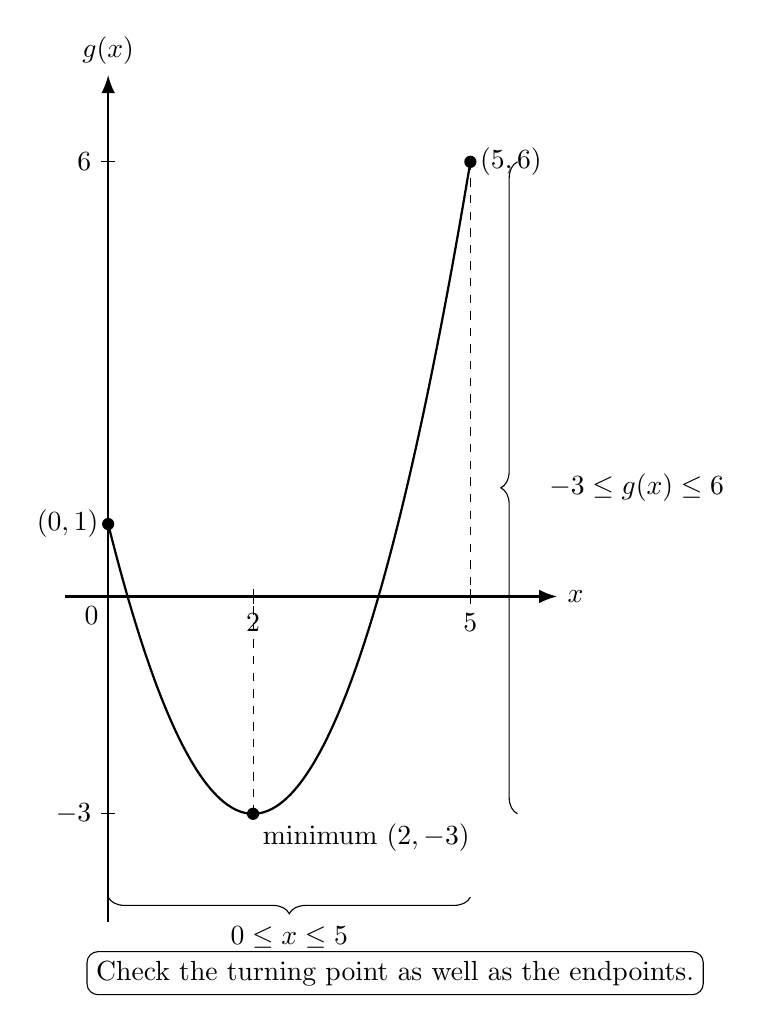
\begin{tikzpicture}[scale=0.92, >=Latex]
\draw[->, thick] (-0.6,0) -- (6.2,0) node[right] {$x$};
\draw[->, thick] (0,-4.5) -- (0,7.2) node[above] {$g(x)$};
\draw[thick, domain=0:5, samples=120] plot (\x,{(\x)^2 - 4*(\x) + 1});
\draw[dashed] (2,-3) -- (2,0);\draw[dashed] (5,6) -- (5,0);\draw[dashed] (0,1) -- (0,0);
\fill (0,1) circle (2.4pt);\fill (2,-3) circle (2.4pt);\fill (5,6) circle (2.4pt);
\node[left] at (0,1) {$(0,1)$};\node[below right] at (2,-3) {minimum $(2,-3)$};\node[right] at (5,6) {$(5,6)$};
\node[below left] at (0,0) {$0$};\draw (2,0.1) -- (2,-0.1) node[below] {$2$};\draw (5,0.1) -- (5,-0.1) node[below] {$5$};
\draw (0.1,-3) -- (-0.1,-3) node[left] {$-3$};\draw (0.1,6) -- (-0.1,6) node[left] {$6$};
\draw[decorate, decoration={brace, mirror, amplitude=6pt}] (0,-4.15) -- (5,-4.15) node[midway, below=7pt] {$0\le x\le5$};
\draw[decorate, decoration={brace, amplitude=6pt}] (5.65,-3) -- (5.65,6) node[midway, right=8pt] {$-3\le g(x)\le6$};
\node[align=left, draw, rounded corners, anchor=west] at (-0.3,-5.2) {Check the turning point as well as the endpoints.};
\end{tikzpicture}
\end{document}
